\section{Motivating Example}
\label{sec:model}

\begin{figure}[h!]
  \vspace*{\beforecaptionskip}
  \centering
  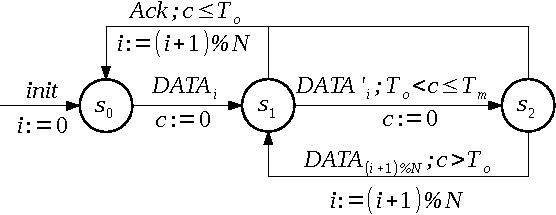
\includegraphics[width=0.6\textwidth]{./figures/dot11_tx_ta.pdf}
  \caption{\textbf{State Machine for 802.11 Transmitter.}}
  \label{fig:dot11_tx_ta}
  \vspace*{\aftercaptionskip}
\end{figure}

Consider the IEEE 802.11 (as known as \wifi{}) transmitter (DUT) state machine
shown in Fig.~\ref{fig:dot11_tx_ta}. After the DUT sends $DATA_i$---a data
packet with sequence number $i$ ($s_0\rightarrow s_1)$, it starts a timer and
wait for the acknowledgment packet---$Ack$. Either it receives $Ack$ within time
$T_o$ ($s_1\rightarrow s_0$), or it sends $DATA'_i$---retransmission of $DATA_i$
($s_1\rightarrow s_2$). Finally, if it still does not receive the $Ack$ packet,
it moves on to next packet\footnote{We assume in this example that the DUT
will retry at most once to succinctly present the state machine.  In practice,
multiple retransmissions will be made before aborting.} ($s_2\rightarrow s_1$).

Obviously, given the DUT's internal log of packet transmission and reception
events, it is trivial to feed such log into the state machine in
Fig.~\ref{fig:dot11_tx_ta} and validate the correctness of DUT's protocol
implementation. In this paper, however, we assume the DUT implementation is a
black box and its internal events are not available. And we seek to validate the
DUT implementation using sniffers.

Two fundamental properties in wireless communication bring uncertainty
to sniffer's observation: packet loss and physical diversity. The sniffer could
either missing packets from the DUT (packet loss), or overhear packets that are
sent to but missed by the DUT (physical diversity).

\begin{figure}[h!]
  \centering
  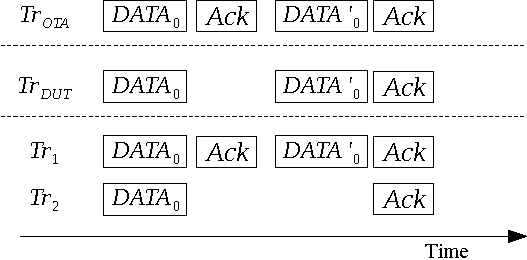
\includegraphics[width=0.6\textwidth]{./figures/false_pos.pdf}
  \caption{\textbf{Uncertainty of Sniffer Observations.} $Tr_{OTA}$ is
    the chronological sequence of packets sent by the DUT and the receiver.
    $Tr_{DUT}$ is DUT's internal events. $Tr_1$ and $Tr_2$ are two possible observations
  of the sniffer.}
  \label{fig:sniffer_in_middle}
\end{figure}

Consider a correct packet exchange sequence and a few sniffer observations
shown in Fig.~\ref{fig:sniffer_in_middle}. The DUT first sends
$DATA_0$.  Suppose the receiver receives $DATA_0$ and sends the $Ack$ which the
DUT does not receive. Eventually the DUT's timer fires and it sends $DATA'_0$.
This time the $DATA'_0$ reaches receiver and the DUT also receives the $Ack$.

In first possible sniffer observation $Tr_1$ where the sniffer \textit{overhears} the
first $Ack$ packet, a validation \textit{uncertainty} arises when the sniffer
sees the $DATA'_0$: was the previous $Ack$ missed by the
DUT or is there a bug in DUT which causes it to retransmit even after receiving
the $Ack$?
Similarly, consider another possible sniffer observation
$Tr_2$ where both the $DATA'_0$ and $Ack$ packets were missed by the sniffer.
During this period of time, it appears the DUT neither receives $Ack$
for $DATA_0$ nor sends $DATA'_0$.
Again, without any additional information it is impossible to disambiguate between the
sniffer missing certain packets and a bug in DUT's retransmission logic.

Informally, the question we set out to answer in this paper is: given the
protocol monitor state machine in Fig.~\ref{fig:dot11_tx_ta} and the sniffer's
observation with inherent uncertainty, how to validate that the DUT behaves as
specified?
